\section{LLM Post-train Mindmap}
\begin{frame}
\begin{figure}
\centering
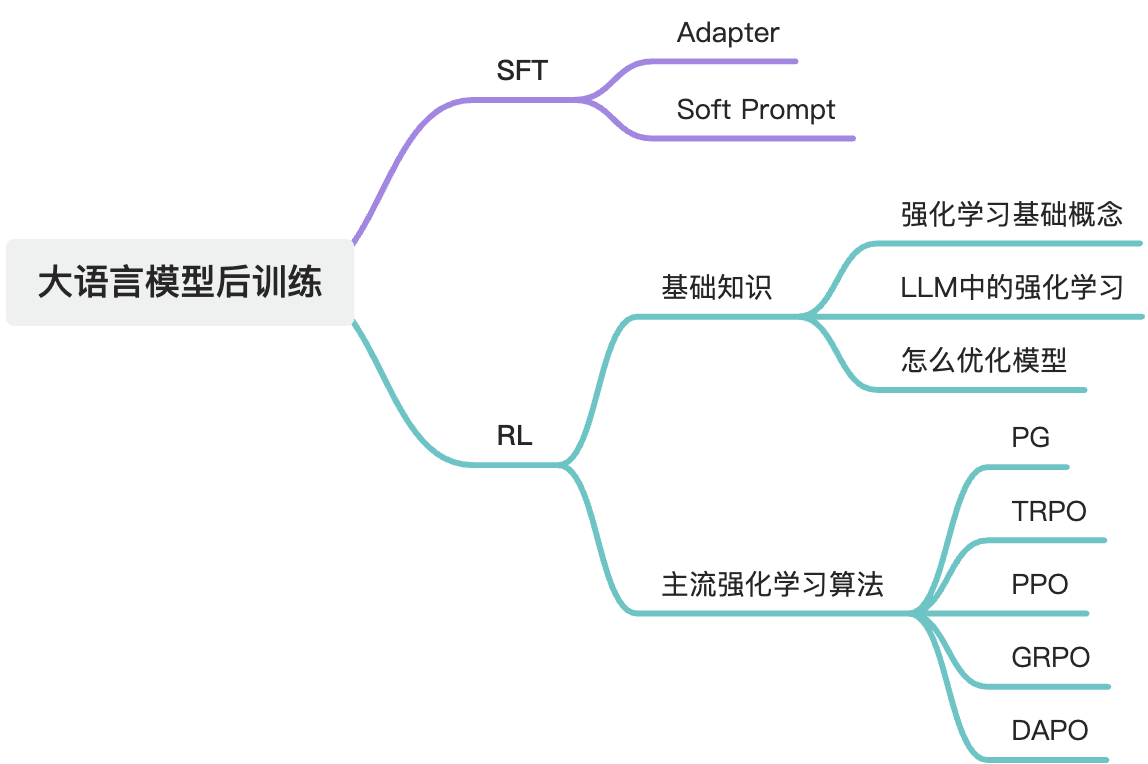
\includegraphics[width=0.9\linewidth]{picture/mindmap.jpg}
\caption{LLM Post-train Mindmap}
\end{figure}
\end{frame}
\section{Supervised Learning Fine-Tuning}
\begin{frame}
Fine-tuning is a type of transfer learning method
\begin{itemize}
\item Supervised domain-specific data
\item Fine-tune the pre-trained model
\item Parameter Efficient Fine-Tuning (PEFT)
\begin{itemize}
\item Adapter-Like methods
\item Soft Prompts
\end{itemize}
\end{itemize}
\begin{figure}
\centering
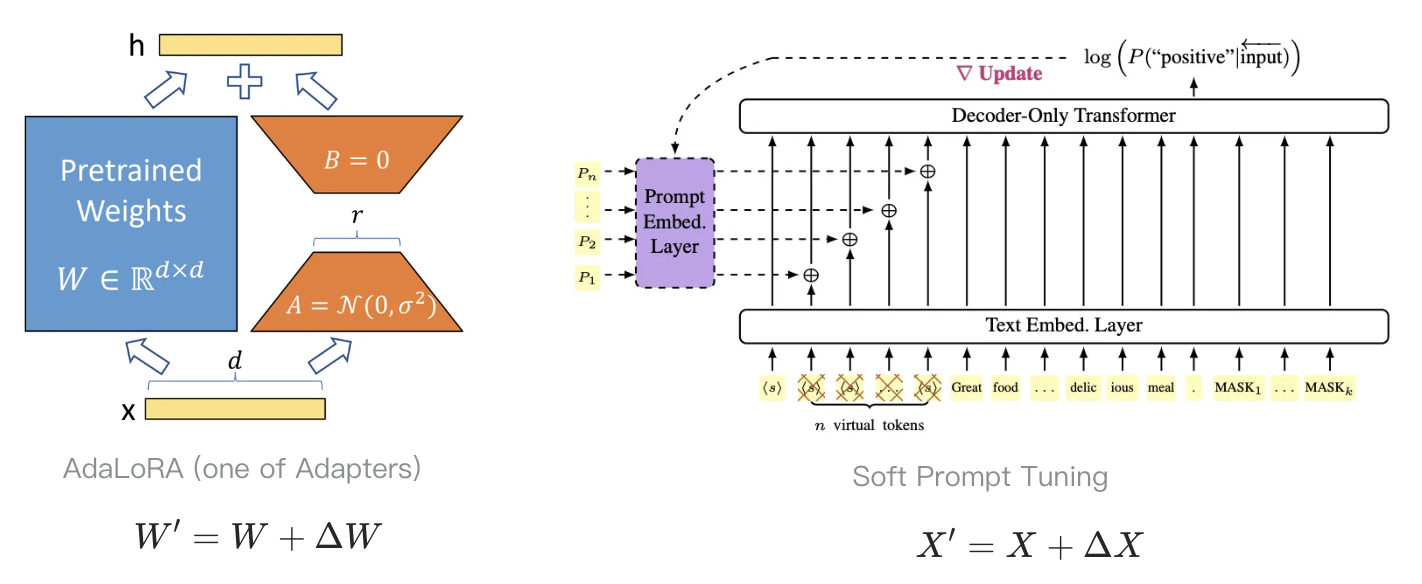
\includegraphics[width=.9\linewidth]{picture/fine_tuning.png}
\caption{Two mainstream fine-tuning methods}
\end{figure}
\end{frame}
\section{Reinforce Learning}
\subsection{Primary}
\subsubsection{Basic Concepts}
\begin{frame}
\textbf{Basic Concepts for RL}:
\begin{itemize}
\item \textit{State}, \textit{Action}, \textit{Reward}
\item  State Transition, Policy $\pi(a|s)$
\begin{figure}
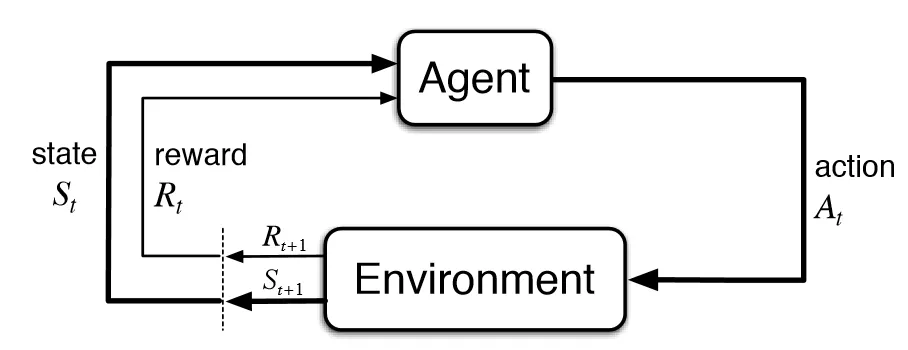
\includegraphics[width=.8\linewidth]{picture/rlsys.png}
\end{figure}
\item Trajectory, Episode, Return (discounted)
\begin{align*}
&s_{1}\xrightarrow[r=0]{a_{2}} s_{2}\xrightarrow[r=0]{a_{3}} s_{5}\xrightarrow[r=0]{a_{3}} s_{8}\xrightarrow[r=1]{a_{2}} s_{9}\xrightarrow[r=1]{a_{5}} s_{9}\xrightarrow[r=1]{a_{5}} s_{9}\ldots
\\
&returns = r_1 + \gamma r_2 + \gamma^2 r_3 + \gamma^3 r_4 + \ldots
\end{align*}
\end{itemize}
\end{frame}
\begin{frame}
\begin{itemize}
\item State Value $v_{\pi}(s)$: Return starting from $s$ under policy $\pi$.
\item Action Value $q_{\pi}(s, a)$: Return starting from $s$ taking action $a$ under policy $\pi$.
$$
v_{\pi}(s) = \sum_{a \in \mathcal{A}} \pi(a|s) q_{\pi}(s, a)
$$
\item Bellman Equation (BE): Describe the recursive relationship of state values.
\end{itemize}
\end{frame}
\begin{frame}
\begin{figure}
\centering
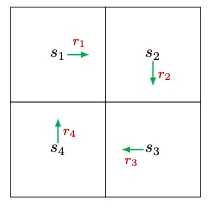
\includegraphics[width=.35\linewidth]{picture/state_transition_example.png}
\caption{Example of state value, action value and  BE}
\end{figure}
\begin{align*}
v_{1} &= r_{1} + \gamma r_{2} + \gamma^{2} r_{3} + \cdots, \\
v_{2} &= r_{2} + \gamma r_{3} + \gamma^{2} r_{4} + \cdots, \\
v_{3} &= r_{3} + \gamma r_{4} + \gamma^{2} r_{1} + \cdots, \\
v_{4} &= r_{4} + \gamma r_{1} + \gamma^{2} r_{2} + \cdots
\end{align*}
\end{frame}
\begin{frame}
Bellman Equation Matrix Form: $v = r + \gamma Pv$
$$
\small
\underbrace{\left[\begin{array}{l}
v_{1} \\
v_{2} \\
v_{3} \\
v_{4}
\end{array}\right]}_{v} =
\left[\begin{array}{l}
r_{1} \\
r_{2} \\
r_{3} \\
r_{4}
\end{array}\right] +
\left[\begin{array}{l}
\gamma v_{2} \\
\gamma v_{3} \\
\gamma v_{4} \\
\gamma v_{1}
\end{array}\right] =
\underbrace{\left[\begin{array}{l}
r_{1} \\
r_{2} \\
r_{3} \\
r_{4}
\end{array}\right]}_{r} +
\gamma \underbrace{\left[\begin{array}{llll}
0 & 1 & 0 & 0 \\
0 & 0 & 1 & 0 \\
0 & 0 & 0 & 1 \\
1 & 0 & 0 & 0
\end{array}\right]}_{P}
\underbrace{\left[\begin{array}{l}
v_{1} \\
v_{2} \\
v_{3} \\
v_{4}
\end{array}\right]}_{v}
$$
Solution:
$$
v = (I - \gamma P)^{-1} r
$$
Insights: current value $v$ depends on the current reward $r$ and
the future value $v$ (rewards).
\end{frame}
\subsubsection{RL with LLM}
\begin{frame}
\frametitle{RL with LLM}
\begin{figure}
\centering
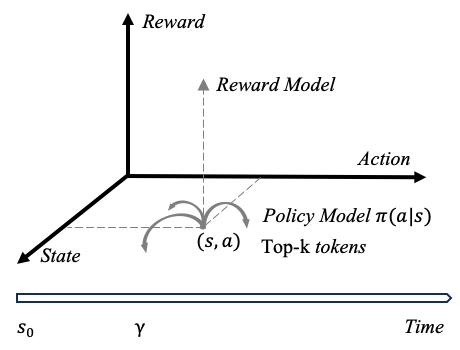
\includegraphics[width=.5\linewidth]{picture/rlsys2.png}
\caption{RL with LLM}
\end{figure}
\begin{itemize}
\item state = context
\item action = next token probability prediction
\item reward = sentence return
\end{itemize}
\end{frame}
\subsubsection{Algorithms}
\begin{frame}
To find Best Policy with Highest state value.
\begin{itemize}
\item Policy Iteration (PI)
\item Value Iteration (VI)
\end{itemize}
\begin{figure}
\centering
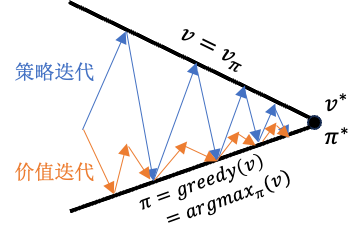
\includegraphics[width = .6\linewidth]{picture/pivi.png}
\caption{Policy iteration and value iteration.}
\end{figure}
\end{frame}
\begin{frame}
\begin{itemize}
\begin{block}{Law of Large Numbers, LLN}
For a random variable $X$, suppose that $\{x_{i}\}_{i=1}^{n}$ are some i.i.d. samples.
$\bar{x}$ is an unbiased estimate of $\mathbb{E}[X]$, and its variance decreases to 0 as $n$ increases to $\infty$.
\end{block}
\item Monte Carlo (MC): Mean estimation. E.g., in PI,
\begin{align*}
v_{\pi_k} &= \sum_{a}\pi(a|s)q_{\pi_k}(s,a)\\
&\approx \sum_{a}\pi(a|s)\left[
\frac{1}{n}\sum_{i=1}^n g_{\pi_k}^{(i)}(s,a),
\right]
\end{align*}
where $g_{\pi_k}^{(i)}(s,a)$ is the $i$-th sampled action values.
\end{itemize}
\end{frame}
\begin{frame}
\begin{itemize}
\item Temporal Difference Method:
\begin{itemize}
\item Given a policy $\pi$, our goal is to estimate $v_{\pi}(s)$ for all $s\in \mathcal{S}$.
And we have some experience samples $(s_0, r_1, s_1, \dots , s_t, r_{t+1}, s_{t+1}, \dots)$.
\item TD algorithm can estimate $v_{\pi}(s)$ using samples
\begin{align*}
\underbrace{v_{t+1}\left(s_{t}\right)}_{\text{new estimate}}
&= \underbrace{v_{t}\left(s_{t}\right)}_{\text{current estimate}} \\
&- \alpha_{t}\left(s_{t}\right)
\Bigg[
\overbrace{
v_{t}\left(s_{t}\right)
-
\Bigg(
\underbrace{r_{t+1} + \gamma v_{t}\left(s_{t+1}\right)}_{\text{TD target } \bar{v}_{t}}
\Bigg)
}^{\text{TD error } \delta_t}
\Bigg]
\\
v_{t+1}(s) &= v_t(s), \text{for all } s \neq s_t,
\end{align*}
\textit{Note}: $v(s_t) = r_t + \gamma r_{t+1} + \gamma^2 r_{t+2} + \dots
= r_t + \gamma (r_{t+1} + \gamma r_{t+2} + \dots) = r_t + \gamma v(s_{t+1})$.
\end{itemize}
\end{itemize}
\end{frame}
\begin{frame}
\begin{block}{Robbins-Monro algorithm}
RM can find the root of the equation
$
g(\omega) = 0,
$
by
\vspace{-3mm}
$$
\omega_{k+1} = \omega_k - \alpha_k
g(\omega_k)
, \text{ where } \alpha_k = \frac{1}{k}.
$$
\end{block}
\begin{figure}
\centering
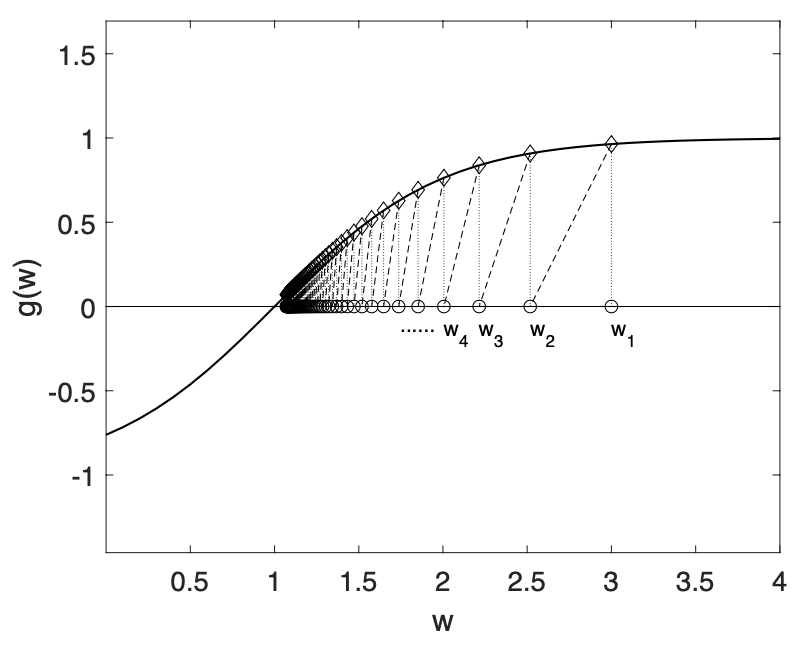
\includegraphics[width=.65\linewidth]{picture/td.png}
\vspace{-2mm}
\caption{Temporal difference learning}
\end{figure}
\end{frame}
\begin{frame}
\begin{block}{Features of MC and TD}
MC: unbias, simple, high variance (need many samples), inefficient online learning.
TD: efficient online learning, low variance, bias, sensitive to hyperparameters.
\end{block}
\begin{itemize}
\item Advantage Estimation: $A_\pi(s,a) = q_\pi(s, a) - v_\pi(s)$
\item Generalized Advantage Estimation, GAE
\begin{itemize}
\item Combinding MC with TD to estimate advantages.
\item Iterative estimation with partial sampling (tradeoff by $\lambda$).
\end{itemize}
\end{itemize}
\end{frame}
\subsection{Policy Gradient}
\begin{frame}
\textbf{Policy Representation}: from discrete to continuous, from table to function.
\begin{itemize}
\item Value-based: $\pi$ is optimized by maximizing $v(s)$ or $q(s,a)$.
e.g., Sarsa, Q-learning.
\item Policy-based: $\pi$ is optimized by certain scalar metrics $J(\theta)$.
e.g., Policy Gradient.
\end{itemize}
\begin{align*}
&\pi_{\theta}^*(a|s) = \arg \max_{\pi_\theta} J(\theta) \\
&\theta_{t+1} = \theta_t + \alpha \nabla_\theta J(\theta_t)
\end{align*}
\begin{block}{Question}
How to define target $J(\theta)$?
\end{block}
\end{frame}
\begin{frame}
\textbf{Policy Gradient, PG}
\begin{block}{Policy Gradient Theorem}
The gradient of $J(\theta)$ is
\begin{align*}
J(\theta) &=
\sum_{s\in \mathcal{S}}\eta(s)\sum_{a \in \mathcal{A}}\pi_\theta(a|s)q_\pi(s,a)\\
&\triangleq \mathbb{E}_{S\sim\eta,A\sim\pi_\theta(S)}\left[
\ln \pi_\theta(A|S)q_\pi(S,A)
\right]
\end{align*}
where $\eta$ is a state distribution.
\end{block}
Parameter updating with SGD:
\begin{align*}
\theta_{t+1} &= \theta_t + \alpha \nabla_\theta J(\theta_t) \\
&=\theta_t + \alpha \nabla_{\theta} \ln \pi_\theta(a_t|s_t)q_\pi(s_t,a_t) \\
&=\theta_t + \alpha \underbrace{\left(
\frac{q_t(s_t, a_t)}{\pi_{\theta_t}(a_t|s_t)}
\right)}_{\beta_t \text{ can be estimated by MC or TD}}
\nabla_\theta \pi_{\theta_t}(a_t|s_t).
\end{align*}
\end{frame}
\subsection{TRPO}
\begin{frame}
\textbf{Trust Region Policy Optimization, TRPO}
\begin{block}{Drawbacks of privious methods}
Complex, sensitive to learning rate...
\end{block}
\begin{itemize}
\item Equivalent Target:
$$
J(\theta) = \mathbb{E}_{S,A \sim \pi_{\text{old}}}\left[
\frac{\pi_\theta(a|s)}{\pi_{\text{old}}(a|s)} A_{\text{old}}(s,a)
\right]
$$
\item Limited Updating: $$
\mathbb{D}_{\text{KL}}(\pi_\theta \| \pi_{\text{old}}) \leq \varepsilon
$$
\textit{Note}: we can describe the ``difference'' between policies by
$$
\mathbb{D}_{\text{KL}}(P\|Q) = \sum_{i=1}^n p(\mathbf{x_i})\ln p(\mathbf{x_i}) - p(\mathbf{x_i}) \ln q(\mathbf{x_i}).
$$
\end{itemize}
\end{frame}
\subsection{PPO}
\begin{frame}
\textbf{Proximal Policy Optimization, PPO}
\begin{block}{Drawbacks of TRPO}
Difficult to explain and adjust.
\end{block}
There are two popular PPO variances:
\begin{itemize}
\item  PPO1: PPO Penality (softer KL):
\begin{align*}
J(\theta) =
\mathbb{E}_{s,a \sim \pi_{\text{old}}}
\left[
\frac{\pi_\theta(a|s)}{\pi_{\text{old}}} A_{\pi_{\text{old}}}(s,a)
\right]
- \beta \mathbb{D}_{\text{KL}}(\pi_{\text{old}}\| \pi_\theta),
\end{align*}
$\beta =2\beta$ if $\mathbb{D}_{\text{KL}} > 1.5\varepsilon$, $\beta=\beta/2$ if $\mathbb{D}_{\text{KL}} < 1.5\varepsilon$
\item PPO2: PPO Clip:
\begin{align*}
\mathbb{E}_{s,a \sim \pi_{\text{old}}}
\left[
\min \left(
\rho A_{\pi_{\text{old}}}(s,a),
clip(\rho, 1 - \varepsilon, 1 + \varepsilon)A_{\pi_{\text{old}}}(s,a)
\right)
\right] ,
\end{align*}
where $\rho = \frac{\pi_\theta(a|s)}{\pi_{\text{old}}}$.
\end{itemize}
\end{frame}
\subsection{GRPO}
\begin{frame}
\textbf{Group Relative Policy Optimization, GRPO}
\begin{figure}
\centering
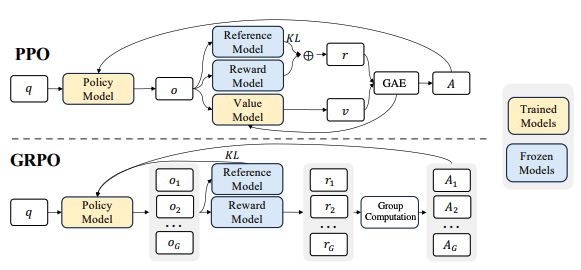
\includegraphics[width=.8\linewidth]{picture/ppo_and_grpo.png}
\caption{PPO and GRPO}
\end{figure}
\vspace{-5mm}
\begin{tiny}
\begin{align*}
J_{\text{PPO}} &=
\mathbb{E}_{q\sim Q, o \sim \pi_{\theta_{\text{old}}}}
\underbrace{\frac{1}{|o|}\sum_{t=1}^{|o|}\min \left[
\rho A_t, clip\left(
\rho, 1-\varepsilon, 1+\varepsilon
\right)A_t
\right]}_{\text{token-by-token advantage estimation}},
\text{ where } A = \texttt{GAE}(r, v). \\
J_{\text{GRPO}} &=
\mathbb{E}_{q\sim Q, o \sim \pi_{\theta_{\text{old}}}}
\underbrace{\frac{1}{G}
\sum_{i=1}^G
\left\{
\frac{1}{|o_i|}\sum_{t=1}^{|o_i|}\min \left[
\rho \hat{A}_t, clip\left(
\rho, 1-\varepsilon, 1+\varepsilon
\right)\hat{A}_t
\right] - \beta \mathbb{D}_{\text{KL}}(\pi_\theta \| \pi_{\text{ref}})
\right\}
}_{\text{group relative advantage estimation}} \\
&\text{ where } \hat{A} = (r - \mathbf{mean}(r))/\textbf{std}(r) \text{ is the normalization of } r.
\end{align*}
\end{tiny}
\end{frame}
\subsection{DAPO}
\begin{frame}
\textbf{Decoupled Clip and Dynamic sAmpling Policy Optimization}
\begin{tiny}
\begin{align*}
J_{\text{DAPO}} &=\mathbb{E}_{q\sim Q, o \sim \pi_{\theta_{\text{old}}}} \\
&\left[
\frac{1}{\sum_{i=1}^{G}|o_i|} \sum_{i=1}^{G}\sum_{t=1}^{|o_i|}
\min \left(
\rho \hat{A}_{i,t}, clip(\rho, 1-\varepsilon_{\text{low}}, 1+\varepsilon_{\text{high}})\hat{A}_{i, t}
\right)
\right]\\
&\text{s.t. } 0 < \left|
\{
o_i \; | \; \textbf{equivalent}(a, o_i)
\}
\right| < G
\end{align*}
\end{tiny}
\begin{itemize}
\item Remove KL due to long CoT reasoning ($\mathbb{D}_{\text{KL}}$ is too high).
\item Clip-Higher: $\varepsilon_{\text{high}}$ promotes the diversity of the system.
\item Dynamic Sampling: $\hat{A}$ is invalid with all samples' accury equal to 1 or 0.
\item Rebalancing Act: GRPO's loss is unfair to long CoT case, since each sample in group is equally weighted.
\end{itemize}
\end{frame}
